\documentclass{beamer}
\usepackage{beamerthemeshadow}

%\documentclass{article}
%\usepackage{beamerarticle}
%\usepackage{graphicx}

\usepackage{lastpage}
\usepackage{xcolor}
\usepackage{pgf}
\usepackage{colortbl}

\newcommand{\bi}{\begin{itemize}}
\newcommand{\ei}{\end{itemize}}
\newcommand{\be}{\begin{enumerate}}
\newcommand{\ee}{\end{enumerate}}
\newcommand{\bd}{\begin{description}}
\newcommand{\ed}{\end{description}}
\newcommand{\prbf}[1]{\textbf{#1}}
\newcommand{\prit}[1]{\textit{#1}}
\newcommand{\beq}{\begin{equation}}
\newcommand{\eeq}{\end{equation}}
\newcommand{\bdm}{\begin{displaymath}}
\newcommand{\edm}{\end{displaymath}}

\newcommand{\ft}[1]{
  \frametitle{\begin{tabular}{p{4.2in}r} \textcolor{white}{#1} & \small{\insertframenumber / \inserttotalframenumber} \end{tabular}}
  \setbeamercovered{transparent=18}
}

\newcommand{\stepinv}{\setbeamercovered{invisible}}
\newcommand{\stopinv}{\setbeamercovered{transparent=18}}
\newcommand{\uncoverinv}[1]
{
  \setbeamercovered{invisible}
  \uncover<+->{#1}
  \setbeamercovered{transparent=18}
}
\newcommand{\ans}[1]{\textcolor{blue}{#1}}
\newcommand{\ansinv}[1]
{
  \setbeamercovered{invisible}
  \uncover<+->{\textcolor{blue}{#1}}
  \setbeamercovered{transparent=18}
}
\newcommand{\setinv}{\setbeamercovered{invisible}}
\newcommand{\setvis}{\setbeamercovered{transparent=18}}
\newcommand{\centerpic}[2]
{
  \begin{center}
  \includegraphics[#1]{#2}
  \end{center}
}
\newcommand{\h}[1]{\hat{#1}}
\newcommand{\ds}{\displaystyle}
\newcommand{\hl}[1]{\alt<#1>{\rowcolor{lightgreen}\hspace{-2.1pt}}{\hspace{-2.1pt}}}

\definecolor{mycolor}{rgb}{0.125,0.5,0.05}
\definecolor{lightgreen}{rgb}{0.54,0.85,0.4}
\usecolortheme[named=mycolor]{structure}

\title[Empirical Significance of Learning with Firm-Specific Capital]{Empirical Significance of Learning in a New Keynesian Model with Firm-Specific Capital}
\author[Job Market Paper. October 2007.]{James Murray\\Indiana University}
\date{October 5, 2007}

\begin{document}

\frame{\titlepage}
\setcounter{framenumber}{0}

\section{}
\subsection{Introduction to Learning}
\frame{
  \ft{Learning vs. Rational Expectations}
  \bi
  \item<+-> Rational Expectations: agents have knowledge of economy's structure, all parameters, distribution of shocks.  
  \item<+-> Learning: Agents form expectations with least squares forecasts.
  \item<+-> Popular assumption: agents use the correct specification.
  \item<+-> Misspecifications:
    \bi
    \item<.-> Some variables in economy are unobservable to agents.
    \item<.-> Agents ignore multi-variate structure, use univariate methods.
    \item<.-> Agents use additional variables.
    \ei
  \ei
}

\frame
{
  \ft{Learning and Monetary Models}
  \bi
  \item<+-> Prolonged inflation following a shock: 
    \bi \item<.-> Orphanides and Williams (RED 2005). \ei
  \item<+-> Bad monetary policy prescriptions:
    \bi \item<.-> Orphanides and Williams (JEDC 2005), Primiceri (QJE 2006). \ei
  \item<+-> Output and inflation persistence: 
    \bi \item<.-> Milani (2005). \ei
  \ei
}

\subsection{Initial Conditions}
\frame
{
  \ft{Initial Conditions}
  \bi
  \item<+-> Initial beliefs can play a major role.
  \item<+-> Orphanides and Williams (JEDC 2005):
    \bi
    \item<.-> Central Bank began under-estimating natural rate of unemployment.
    \ei
  \item<+-> Primiceri:
    \bi
    \item<.-> Central Bank began under-estimating unemployment and inflation persistence.
    \ei
  \item<+-> Milani:
    \bi
    \item<.-> Many initial beliefs set to pre-sample VAR(1).
    \item<.-> Assumes lower inflation persistence, sensitivity of output to inflation.
    \item<.-> Assumes shocks are observable, sets initial impacts to zero.
    \ei 
  \item<+-> Missing from empirical literature:
    \bi
    \item<.-> Systematic way for specifying initial conditions.
    \item<.-> Estimate initial conditions.
    \item<.-> Sensitivity analysis to initial conditions.
    \ei
  \ei
}

\frame
{
  \ft{Strategies for Initial Conditions}
  \bi
  \item<+-> Use the rational expectations solution.
    \bi
    \item<.-> Benefit: Initial conditions are consistent with model.
    \item<.-> Draw back: Learning dynamics are small near the RE equilibrium. (Williams 2003).
    \ei
  \item<+-> Assume limited information set.
    \bi
    \item<.-> Agents cannot observe realizations of stochastic shocks.
    \item<.-> Initialize beliefs of remaining coefficients equal to RE solution.
    \item<.-> Benefit: more realistic.
    \ei
  \item<+-> Using limited information, set initial beliefs to pre-sample least squares estimates.
    \bi
    \item<.-> Benefit: Most likely to mirror actual beliefs.
    \item<.-> Draw back: sometimes so far from RE the learning model is unstable (Slobodyan and Wouters 2007).
    \ei
  \item<+-> Jointly estimate initial conditions.
    \bi
    \item<.-> Draw back: many additional parameters, over-fitting problem.
    \ei
  \ei
}

\section{Learning}
\subsection{General Models}
\frame
{
  \ft{General Form}
  \bi
  \item<+-> Linear Dynamic Stochastic General Equilibrium models:
  \uncover<.->{\bdm \Omega_{0} x_t = \Omega_{1} x_{t-1} + \Omega_{2} E_t^* x_{t+1} + \Psi v_t \edm}
  \uncover<.->{\bdm v_t = A v_{t-1} + \epsilon_t \edm}
    \bi
    \item<+-> $x_t$ vector of time $t$ macroeconomic variables, observable to agents at following time period.
    \item<+-> $z_t$: vector of time $t$ shocks, possibly observable to agents in current period.
    \ei
  \item<+-> Rational expectations solution:
  \uncover<.->{\bdm x_{t} = G x_{t-1} + M v_{t} \edm}
  \ei
}

\frame
{
  \ft{Learning}
  \bi
  \item<+-> Agents estimate elements of $G$ and $M$ by least squares.
  \item<+-> Information at available at time $t$: $x_{t-1}$, $v_t$:
    \bi
    \item<+-> $X_t$: vector of regressors: $X_t' = [1~ x_{t-2}'~ v_{t-1}']$.
    \item<.-> $Y_t$: vector of dependent variables: $Y_t = x_{t-1}$.
    \ei
  \item<+-> When $v_t$ is observable, I suppose agents know $A$.
  \item<+-> Let $\Phi_t$ vector of least squares estimates of the coefficients in matrices $G$ and $M$.
  \item<+-> Ordinary Least Squares estimate of $\phi_t$:
  \uncover<.->{\bdm \label{eq:Phi} \Phi_t' = \left( \frac{1}{t-1} \sum_{\tau=2}^{t} X_{\tau} X_{\tau}' \right)^{-1} \left( \frac{1}{t-1} \sum_{\tau=2}^{t} X_{\tau} Y_{\tau}' \right) \edm}
  \ei
}

\subsection{Learning Algorithm}
\frame
{
  \ft{Learning Algorithm}
  \bi
  \item<+-> Recursive form:
  \uncover<+->{\bdm \label{eq:lnPhi} \Phi_t = \Phi_{t-1} + g_t (Y_{t} - \Phi_{t-1} X_{t}) X_{t}' R_t^{-1}\edm}
  \uncover<+->{\bdm \label{eq:lnR} R_t = R_{t-1} + g_t (X_{t} X_{t}' - R_{t-1})\edm}
    \bi \item<+-> Where $g_t = 1/(t-1)$. \ei
  \item<+-> OLS learning: dynamics disappear in the long run.
  \item<+-> Constant gain learning: $g_t = g$.
  \ei
}

\subsection{Constant Gain Learning}
\frame
{
  \ft{Motivation for Constant Gain Learning}
  \bi
  \item<+-> Learning dynamics persist in the long run.
  \item<+-> Reasonable approximation to a rolling window estimation procedure.
    \bi
    \item<.-> Typically 30-50 year windows are used in forecasting quarterly macroeconomic variables.
    \item<+-> Johnston Williamson (2007): data available for U.S. output and price level back to 1790.
    \ei
  \item<+-> Swanson and White (RES 1997):
    \bi
    \item<+-> Adaptive estimation procedures out-perform non-adaptive procedures.
    \item<+-> Multivariate procedures out-perform univariate procedures.
    \item<+-> Linear models out-perform non-linear models.
    \item<+-> Adaptive, multivariate, linear models outperform professional forecast surveys.
    \ei
  \ei
}

\section{Model}
\subsection{Standard Model}
\frame
{
  \ft{New Keynesian Monetary Model}
  \bi
  \item<+-> Examine two popular specifications
    \be
    \item<+-> Standard three equation model: IS equation, Phillips curve, monetary policy.  Woodford (2003).
    \item<+-> Add endogenous capital.  Woodford (IJCB 2005).
    \ee
  \item<+-> Details behind IS equation:
    \bi
    \item<.-> Utility maximizing consumers.
    \item<.-> Habit formation in utility function (source of persistence).
    \item<.-> Intertemporal substitution.
    \item<.-> Goods market clearing.
    \ei
  \item<+-> Details behind the Phillips curve:
    \bi
    \item<.-> Profit maximizing firms.
    \item<.-> Sticky prices.
    \item<.-> Price indexation (source of persistence). 
    \item<.-> Labor market clearing.
    \ei
  \item<+-> Monetary Policy (Taylor rule):
    \bi
    \item<.-> Interest rate set in respond to output gap, inflation, past interest rate.
    \ei
  \ei
}

\subsection{Firm Specific Capital}
\frame
{
  \ft{Firm Specific Capital}
  \bi
  \item<+-> Output is produced with labor and capital.
  \item<+-> Investment is subject to adjustment cost.
  \item<+-> Capital depreciates at a constant rate.
  \item<+-> Firm specific capital
    \bi
    \item<+-> No perfect capital rental market.
    \item<+-> Capital cannot be transfered between firms.
    \item<+-> Individual capital stocks affect an individual firm's marginal costs.
    \ei
  \ei
}

\subsection{Stochastic shocks}
\frame
{
  \ft{Stochastic shocks}
  \bi
  \item<+-> Specification 1: Three equation model (without capital)
    \bi
    \item<.-> Natural interest rate shock.
    \item<.-> Cost-push shock.
    \item<.-> Monetary policy shock.
    \ei
  \item<+-> Specification 2: Model with capital
    \bi
    \item<.-> Preference shock.
    \item<.-> Technology shock.
    \item<.-> Investment technology shock.
    \item<.-> Monetary policy shock.
    \ei
  \ei
}

\section{Estimation}
\subsection{Five Cases}
\frame
{
  \ft{Five Expectations Frameworks}
  \bi
  \item<+-> Estimate two NK specifications by maximum likelihood.
  \item<+-> For each specification, estimate five expectations frameworks: 
    \be
    \item<+-> Rational Expectations
    \item<+-> Learning with RE solution for initial $\Phi_t$, $R_t$.
    \item<+-> Learning with limited information set.
      \bi
      \item<.-> Shocks are unobservable.
      \item<.-> Initial coefficients on remaining variables set equal to RE solution.
      \ei
    \item<+-> Limited information set with pre-sample coefficients.
    \item<+-> Limited information set with estimated initial conditions.
    \ee
  \ei
}

\subsection{Pre-sample Initial Conditions}
\frame
{
  \ft{Pre-sample Initial Conditions}
  \bi
  \item<+-> Learning algorithm for constant gain least squares:
  \uncover<+->{\bdm \label{eq:Phisum} \Phi_t = \left( \sum_{\tau=0}^{t-1} \left(1-g\right)^t X_{t-\tau} X_{t-\tau}' \right)^{-1} \left( \sum_{\tau=0}^{t-1} \left(1-g\right)^{\tau} X_{t-\tau} Y_{t-\tau}' \right)\edm}
  \item<+-> Learning gain $g$ estimated jointly with parameters of New Keynesian model.
  \ei
}

\frame
{
  \ft{Pre-sample Initial Conditions}
  \bi
  \item<+-> Specification 1: 
    \bi
    \item<+-> $Y_t$ vector includes output gap, inflation rate, federal funds rate.
    \item<+-> $X_t$ vector includes constant, previous period's output gap, inflation rate, federal funds rate.. 
    \ei
  \item<+-> Specification 2:
    \bi
    \item<+-> $Y_t$ vector includes consumption, capital stock, inflation rate, federal funds rate.
    \item<+-> $X_t$ vector includes constant, previous period's consumption, capital stock, inflation rate, federal funds rate.
    \item<+-> All these variables expressed as percentage deviation from the steady state.
    \item<+-> Data on capital stock constructed using data on investment. 
    \ei
  \ei
}

\subsection{Data}
\frame
{
  \ft{Data}
  \bi
  \item<+-> Quarterly data for 1960:Q1 through 2005:Q4.
  \item<+-> Pre-sample data: Quarterly data for 1954:Q1 through 1959:Q4.
  \item<+-> Specification 1: Model with no capital: 
    \bi
    \item<.-> CBO measure of the output gap.
    \item<.-> Annualized quarterly inflation rate of the GDP deflater.
    \item<.-> Annualized quarterly federal funds rate.
    \ei
  \item<+-> Specification 2: Endogenous capital:
    \bi
    \item<.-> Real private consumption expenditures per capita.
    \item<.-> Real gross private domestic investment per capita.
    \item<.-> Output is defined as the sum of consumption and investment.
    \item<.-> Annualized quarterly inflation rate of the GDP deflator.
    \item<.-> Annualized quarterly federal funds rate.
    \ei
  \item<+-> Consumption and Investment: trend growth rate removed.
  \ei
}

\section{Results}
\subsection{Model Without Capital}
\frame
{
\ft{No Capital: RE vs. Learning (RE Init.)}
\vspace*{-.15in}
\begin{center}
\begin{scriptsize}
\begin{tabular}{|l|c|rr|rr|} \hline
 & & \multicolumn{2}{|c|}{Case 1} & \multicolumn{2}{|c|}{Case 2} \\ \hline
Description & Parameter & Estimate & Std. Dev. & Estimate & Std. Dev. \\ \hline
Habit Formation & $\eta$ & 0.4221 & 0.1062 & 0.4241 & 0.1216 \\
Inverse IES & $\sigma$ & 0.5152 & 0.4401 & 0.5236 & 0.4865 \\
Phillips Slope & $\kappa$ & 0.0001 & 0.0002 & 0.0001 & 0.0002 \\
Price Indexation & $\gamma$ & 0.9900 & 0.0634 & 0.9901 & 0.0907 \\
MP Persistence & $\rho_r$ & 0.9207 & 0.0207 & 0.9207 & 0.0214 \\
MP Output & $\psi_y$ & 0.4946 & 0.1901 & 0.4949 & 0.1967 \\
MP Inflation & $\psi_{\pi}$ & 1.9994 & 0.0000 & 1.9995 & 0.0000 \\
Nat. Rate Pers. & $\rho_{n}$ & 0.8488 & 0.0684 & 0.8489 & 0.0645 \\
Cost Push Pers. & $\rho_u$ & 0.0000 & 0.0692 & 0.0000 & 0.0608 \\
Nat. Rate Std. Dev. & $\sigma_{n}$ & 0.0751 & 0.0706 & 0.0736 & 0.0741 \\
Cost Push Std. Dev. & $\sigma_{u}$ & 0.0029 & 0.0002 & 0.0029 & 0.0003 \\
MP Std. Dev. & $\sigma_r$ & 0.0030 & 0.0001 & 0.0030 & 0.0001 \\
SS Inflation & $\pi^{*}$ & 5.9904 & 1.2374 & 5.9905 & 1.2739 \\
\hl{2}
Learning Gain & $g$ & -- & -- & 0.0067 & 0.0070 \\\hline 
\multicolumn{2}{|l|}{\hl{3}Log-likelihood} & \multicolumn{2}{|r|}{\hl{3}-459.9390} & \multicolumn{2}{|r|}{\hl{3}-459.5154} \\ 
\multicolumn{2}{|l|}{\hl{3}MSE Output Gap} & \multicolumn{2}{|r|}{\hl{3}0.6087} & \multicolumn{2}{|r|}{\hl{3}0.6061} \\ 
\multicolumn{2}{|l|}{\hl{3}MSE Inflation} & \multicolumn{2}{|r|}{\hl{3}1.3313} & \multicolumn{2}{|r|}{\hl{3}1.3269} \\ 
\multicolumn{2}{|l|}{\hl{3}MSE Fed. Funds Rate} & \multicolumn{2}{|r|}{\hl{3}1.6480} & \multicolumn{2}{|r|}{\hl{3}1.6519} \\ \hline 
\end{tabular}
\end{scriptsize}
\end{center}
}

\frame
{
  \ft{No Capital: Forecast Errors}
\begin{tabular}{ccc}
\multicolumn{3}{c}{Rational Expectations} \\ 
Output gap & Inflation & Fed Funds Rate \\ 
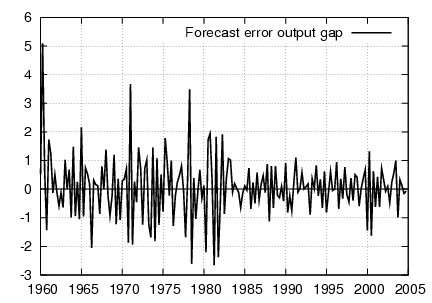
\includegraphics[scale=0.17]{/home/jmmurray/workspace/code/cfortran/re_Forecast_error_output_gap.png} & 
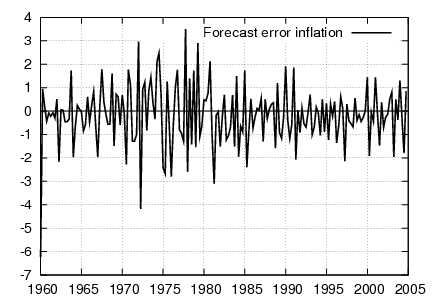
\includegraphics[scale=0.17]{/home/jmmurray/workspace/code/cfortran/re_Forecast_error_inflation.png} & 
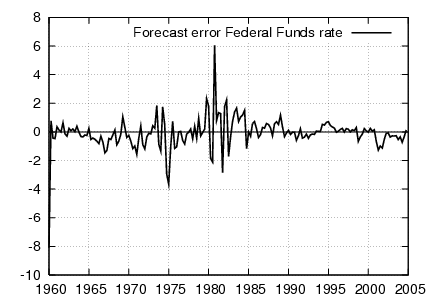
\includegraphics[scale=0.17]{/home/jmmurray/workspace/code/cfortran/re_Forecast_error_Federal_Funds_rate.png} \\ \\ 
\multicolumn{3}{c}{Learning with RE Initial Conditions} \\ 
Output gap (0.9993) & Inflation (0.9973) & Fed Funds Rate (0.9999) \\ 
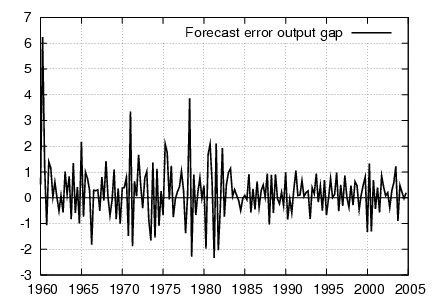
\includegraphics[scale=0.17]{/home/jmmurray/workspace/code/cfortran/initre_Forecast_error_output_gap.png} & 
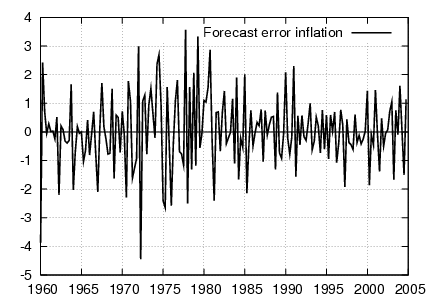
\includegraphics[scale=0.17]{/home/jmmurray/workspace/code/cfortran/initre_Forecast_error_inflation.png} & 
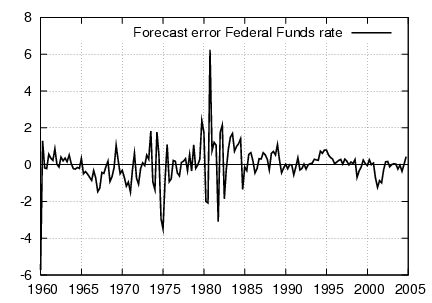
\includegraphics[scale=0.17]{/home/jmmurray/workspace/code/cfortran/initre_Forecast_error_Federal_Funds_rate.png} \\
\end{tabular}
}

\frame
{
\ft{No Capital: RE vs. Learning (Unobservable Shocks)}
\vspace*{-.15in}
\begin{center}
\begin{scriptsize}
\begin{tabular}{|l|c|rr|rr|} \hline
 & & \multicolumn{2}{|c|}{Case 1} & \multicolumn{2}{|c|}{Case 3} \\ \hline
Description & Parameter & Estimate & Std. Dev. & Estimate & Std. Dev. \\ \hline
Habit Formation & $\eta$ & 0.4221 & 0.1062 & 0.3027 & 0.1216 \\
\hl{3}
Inverse IES & $\sigma$ & 0.5152 & 0.4401 & 0.2251 & 0.4865 \\
Phillips Slope & $\kappa$ & 0.0001 & 0.0002 & 0.0004 & 0.0002 \\
Price Indexation & $\gamma$ & 0.9900 & 0.0634 & 0.9999 & 0.0907 \\
MP Persistence & $\rho_r$ & 0.9207 & 0.0207 & 0.9131 & 0.0214 \\
MP Output & $\psi_y$ & 0.4946 & 0.1901 & 0.4762 & 0.1967 \\
MP Inflation & $\psi_{\pi}$ & 1.9994 & 0.0000 & 1.9865 & 0.0000 \\
Nat. Rate Pers. & $\rho_{n}$ & 0.8488 & 0.0684 & 0.8413 & 0.0645 \\
Cost Push Pers. & $\rho_u$ & 0.0000 & 0.0692 & 0.0002 & 0.0608 \\
\hl{3}
Nat. Rate Std. Dev. & $\sigma_{n}$ & 0.0751 & 0.0706 & 0.2736 & 0.0741 \\
Cost Push Std. Dev. & $\sigma_{u}$ & 0.0029 & 0.0002 & 0.0054 & 0.0003 \\
MP Std. Dev. & $\sigma_r$ & 0.0030 & 0.0001 & 0.0030 & 0.0001 \\
SS Inflation & $\pi^{*}$ & 5.9904 & 1.2374 & 5.9539 & 1.2739 \\
\hl{2}
Learning Gain & $g$ & -- & -- & 0.0042 & 0.0070 \\\hline 
\multicolumn{2}{|l|}{\hl{4}Log-likelihood} & \multicolumn{2}{|r|}{\hl{4}-459.9390} & \multicolumn{2}{|r|}{\hl{4}-458.8326} \\ 
\multicolumn{2}{|l|}{\hl{4}MSE Output Gap} & \multicolumn{2}{|r|}{\hl{4}0.6087} & \multicolumn{2}{|r|}{\hl{4}0.6032} \\ 
\multicolumn{2}{|l|}{\hl{4}MSE Inflation} & \multicolumn{2}{|r|}{\hl{4}1.3313} & \multicolumn{2}{|r|}{\hl{4}1.3371} \\ 
\multicolumn{2}{|l|}{\hl{4}MSE Fed. Funds Rate} & \multicolumn{2}{|r|}{\hl{4}1.6480} & \multicolumn{2}{|r|}{\hl{4}1.6378} \\ \hline 
\end{tabular}
\end{scriptsize}
\end{center}
}

\frame
{
  \ft{No Capital: Forecast Errors}
\begin{tabular}{ccc}
\multicolumn{3}{c}{Rational Expectations} \\ 
Output gap & Inflation & Fed Funds Rate \\ 
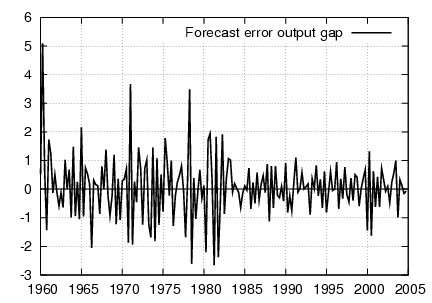
\includegraphics[scale=0.17]{/home/jmmurray/workspace/code/cfortran/re_Forecast_error_output_gap.png} & 
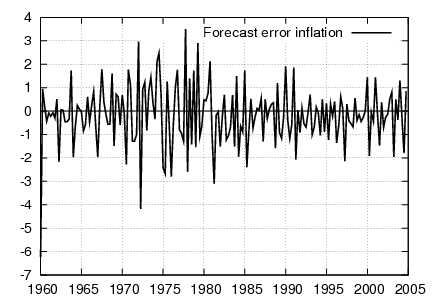
\includegraphics[scale=0.17]{/home/jmmurray/workspace/code/cfortran/re_Forecast_error_inflation.png} & 
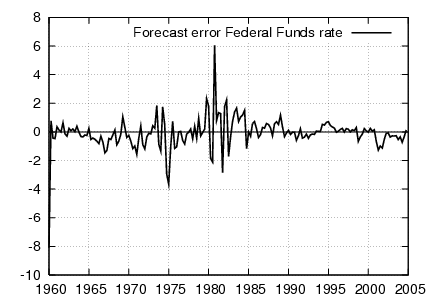
\includegraphics[scale=0.17]{/home/jmmurray/workspace/code/cfortran/re_Forecast_error_Federal_Funds_rate.png} \\ \\ 
\multicolumn{3}{c}{Learning Without Observable Shocks} \\ 
Output gap (0.9846) & Inflation (0.9960) & Fed Funds Rate (0.9996) \\ 
\includegraphics[scale=0.17]{/home/jmmurray/workspace/code/cfortran/initreg_Forecast_error_output_gap.png} & 
\includegraphics[scale=0.17]{/home/jmmurray/workspace/code/cfortran/initreg_Forecast_error_inflation.png} & 
\includegraphics[scale=0.17]{/home/jmmurray/workspace/code/cfortran/initreg_Forecast_error_Federal_Funds_rate.png} \\ \\ 
\end{tabular}
}

\frame
{
\ft{No Capital: RE vs. Learning (Pre-sample init.)}
\vspace*{-.15in}
\begin{center}
\begin{scriptsize}
\begin{tabular}{|l|c|rr|rr|} \hline
 & & \multicolumn{2}{|c|}{Case 1} & \multicolumn{2}{|c|}{Case 4} \\ \hline
Description & Parameter & Estimate & Std. Dev. & Estimate & Std. Dev. \\ \hline
Habit Formation & $\eta$ & 0.4221 & 0.1062 & 0.5293 & 0.1216 \\
\hl{3}
Inverse IES & $\sigma$ & 0.5152 & 0.4401 & 0.2502 & 0.4865 \\
Phillips Slope & $\kappa$ & 0.0001 & 0.0002 & 0.0064 & 0.0002 \\
Price Indexation & $\gamma$ & 0.9900 & 0.0634 & 0.9989 & 0.0907 \\
MP Persistence & $\rho_r$ & 0.9207 & 0.0207 & 0.8454 & 0.0214 \\
MP Output & $\psi_y$ & 0.4946 & 0.1901 & 0.3200 & 0.1967 \\
MP Inflation & $\psi_{\pi}$ & 1.9994 & 0.0000 & 1.5109 & 0.0000 \\
Nat. Rate Pers. & $\rho_{n}$ & 0.8488 & 0.0684 & 0.6810 & 0.0645 \\
\hl{3}
Cost Push Pers. & $\rho_u$ & 0.0000 & 0.0692 & 0.4419 & 0.0608 \\
\hl{3}
Nat. Rate Std. Dev. & $\sigma_{n}$ & 0.0751 & 0.0706 & 0.5835 & 0.0741 \\
\hl{3}
Cost Push Std. Dev. & $\sigma_{u}$ & 0.0029 & 0.0002 & 0.0086 & 0.0003 \\
MP Std. Dev. & $\sigma_r$ & 0.0030 & 0.0001 & 0.0030 & 0.0001 \\
SS Inflation & $\pi^{*}$ & 5.9904 & 1.2374 & 5.8862 & 1.2739 \\
\hl{2}
Learning Gain & $g$ & -- & -- & 0.0828 & 0.0070 \\\hline 
\multicolumn{2}{|l|}{\hl{4}Log-likelihood} & \multicolumn{2}{|r|}{\hl{4}-459.9390} & \multicolumn{2}{|r|}{\hl{4}-573.3274} \\ 
\multicolumn{2}{|l|}{\hl{4}MSE Output Gap} & \multicolumn{2}{|r|}{\hl{4}0.6087} & \multicolumn{2}{|r|}{\hl{4}0.7989} \\ 
\multicolumn{2}{|l|}{\hl{4}MSE Inflation} & \multicolumn{2}{|r|}{\hl{4}1.3313} & \multicolumn{2}{|r|}{\hl{4}2.7104} \\ 
\multicolumn{2}{|l|}{\hl{4}MSE Fed. Funds Rate} & \multicolumn{2}{|r|}{\hl{4}1.6480} & \multicolumn{2}{|r|}{\hl{4}1.7396} \\ \hline 
\end{tabular}
\end{scriptsize}
\end{center}
}

\frame
{
  \ft{No Capital: Forecast Errors}
\begin{tabular}{ccc}
\multicolumn{3}{c}{Rational Expectations} \\ 
Output gap & Inflation & Fed Funds Rate \\ 
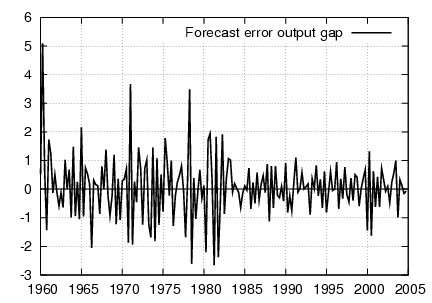
\includegraphics[scale=0.17]{/home/jmmurray/workspace/code/cfortran/re_Forecast_error_output_gap.png} & 
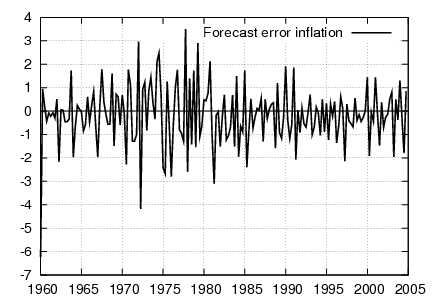
\includegraphics[scale=0.17]{/home/jmmurray/workspace/code/cfortran/re_Forecast_error_inflation.png} & 
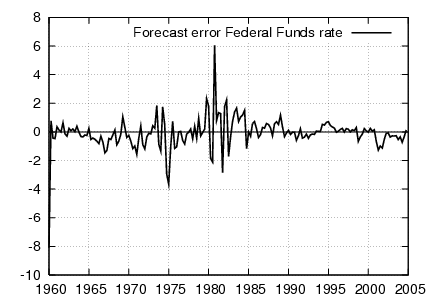
\includegraphics[scale=0.17]{/home/jmmurray/workspace/code/cfortran/re_Forecast_error_Federal_Funds_rate.png} \\ \\ 
\multicolumn{3}{c}{Learning with Pre-sample Initial Conditions} \\ 
Output gap (0.7344) & Inflation (0.7617) & Fed Funds Rate (0.9481) \\ 
\includegraphics[scale=0.17]{/home/jmmurray/workspace/code/cfortran/initwls_Forecast_error_output_gap.png} & 
\includegraphics[scale=0.17]{/home/jmmurray/workspace/code/cfortran/initwls_Forecast_error_inflation.png} & 
\includegraphics[scale=0.17]{/home/jmmurray/workspace/code/cfortran/initwls_Forecast_error_Federal_Funds_rate.png} \\ \\ 
\end{tabular}
}

\frame
{
\ft{No Capital: RE vs. Learning (Pre-sample init.)}
\vspace*{-.15in}
\begin{center}
\begin{scriptsize}
\begin{tabular}{|l|c|rr|rr|} \hline
 & & \multicolumn{2}{|c|}{Case 1} & \multicolumn{2}{|c|}{Case 5} \\ \hline
Description & Parameter & Estimate & Std. Dev. & Estimate & Std. Dev. \\ \hline
Habit Formation & $\eta$ & 0.4221 & 0.1062 & 0.3052 & 0.1216 \\
\hl{2}
Inverse IES & $\sigma$ & 0.5152 & 0.4401 & 0.1960 & 0.4865 \\
Phillips Slope & $\kappa$ & 0.0001 & 0.0002 & 0.0001 & 0.0002 \\
Price Indexation & $\gamma$ & 0.9900 & 0.0634 & 0.9893 & 0.0907 \\
MP Persistence & $\rho_r$ & 0.9207 & 0.0207 & 0.9193 & 0.0214 \\
MP Output & $\psi_y$ & 0.4946 & 0.1901 & 0.4944 & 0.1967 \\
MP Inflation & $\psi_{\pi}$ & 1.9994 & 0.0000 & 1.9992 & 0.0000 \\
Nat. Rate Pers. & $\rho_{n}$ & 0.8488 & 0.0684 & 0.8488 & 0.0645 \\
Cost Push Pers. & $\rho_u$ & 0.0000 & 0.0692 & 0.0000 & 0.0608 \\
\hl{2}
Nat. Rate Std. Dev. & $\sigma_{n}$ & 0.0751 & 0.0706 & 0.2310 & 0.0741 \\
Cost Push Std. Dev. & $\sigma_{u}$ & 0.0029 & 0.0002 & 0.0054 & 0.0003 \\
MP Std. Dev. & $\sigma_r$ & 0.0030 & 0.0001 & 0.0030 & 0.0001 \\
SS Inflation & $\pi^{*}$ & 5.9904 & 1.2374 & 5.9894 & 1.2739 \\
\hl{1}
Learning Gain & $g$ & -- & -- & 0.0000 & 0.0070 \\\hline 
\multicolumn{2}{|l|}{\hl{3}Log-likelihood} & \multicolumn{2}{|r|}{\hl{3}-459.9390} & \multicolumn{2}{|r|}{\hl{3}-449.3276} \\ 
\multicolumn{2}{|l|}{\hl{3}MSE Output Gap} & \multicolumn{2}{|r|}{\hl{3}0.6087} & \multicolumn{2}{|r|}{\hl{3}0.5679} \\ 
\multicolumn{2}{|l|}{\hl{3}MSE Inflation} & \multicolumn{2}{|r|}{\hl{3}1.3313} & \multicolumn{2}{|r|}{\hl{3}1.2922} \\ 
\multicolumn{2}{|l|}{\hl{3}MSE Fed. Funds Rate} & \multicolumn{2}{|r|}{\hl{3}1.6480} & \multicolumn{2}{|r|}{\hl{3}1.6486} \\ \hline 
\end{tabular}
\end{scriptsize}
\end{center}
}

\frame
{
  \ft{No Capital: Forecast Errors}
\begin{tabular}{ccc}
\multicolumn{3}{c}{Rational Expectations} \\ 
Output gap & Inflation & Fed Funds Rate \\ 
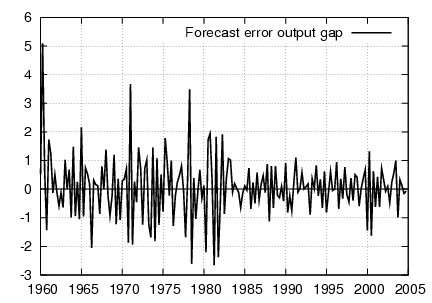
\includegraphics[scale=0.17]{/home/jmmurray/workspace/code/cfortran/re_Forecast_error_output_gap.png} & 
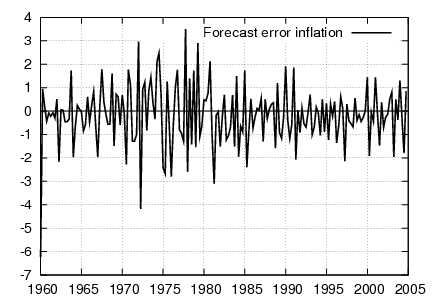
\includegraphics[scale=0.17]{/home/jmmurray/workspace/code/cfortran/re_Forecast_error_inflation.png} & 
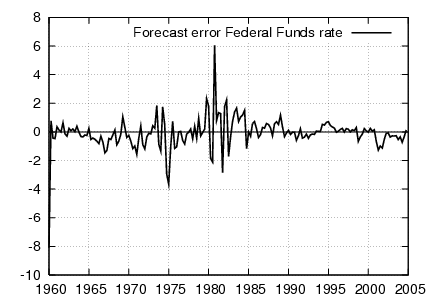
\includegraphics[scale=0.17]{/home/jmmurray/workspace/code/cfortran/re_Forecast_error_Federal_Funds_rate.png} \\ \\ 
\multicolumn{3}{c}{Learning with Estimated Initial Conditions} \\ 
Output gap (0.9682) & Inflation (0.9896) & Fed Funds Rate (0.9997) \\ 
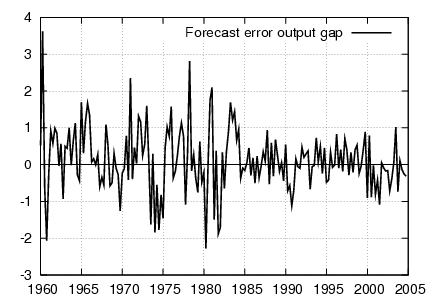
\includegraphics[scale=0.17]{/home/jmmurray/workspace/code/cfortran/initest_Forecast_error_output_gap.png} & 
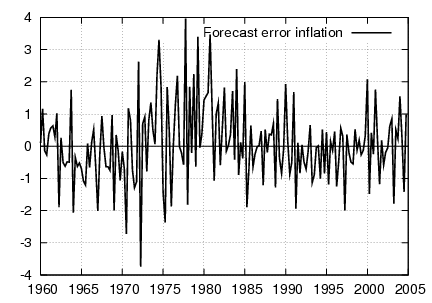
\includegraphics[scale=0.17]{/home/jmmurray/workspace/code/cfortran/initest_Forecast_error_inflation.png} & 
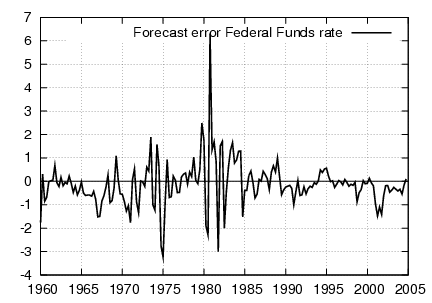
\includegraphics[scale=0.17]{/home/jmmurray/workspace/code/cfortran/initest_Forecast_error_Federal_Funds_rate.png} \\ \\ 
\end{tabular}
}

\subsubsection{Evolution of Shocks}

\frame
{
  \ft{No Capital: Evolution of Shocks}
\begin{tabular}{ccc}
\multicolumn{3}{c}{Rational Expectations} \\ 
Nat. Rate & Cost Push & Policy Shock \\ 
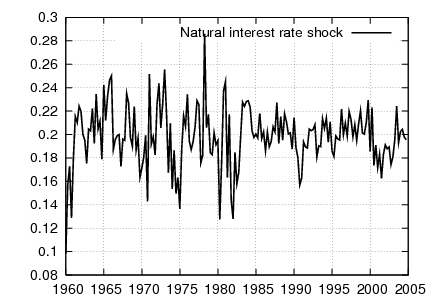
\includegraphics[scale=0.17]{/home/jmmurray/workspace/code/cfortran/re_natint.png} & 
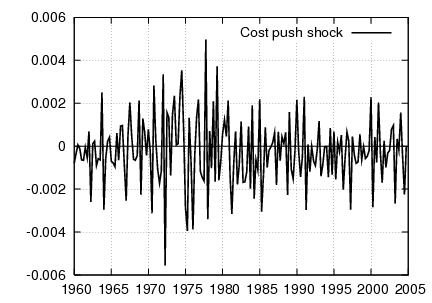
\includegraphics[scale=0.17]{/home/jmmurray/workspace/code/cfortran/re_costpush.png} & 
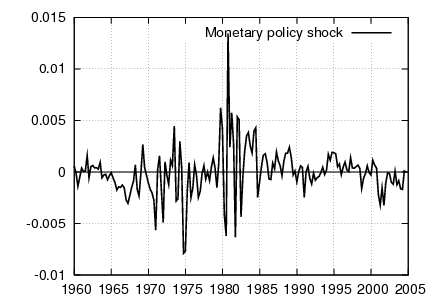
\includegraphics[scale=0.17]{/home/jmmurray/workspace/code/cfortran/re_mpshock.png} \\ \\ 
\multicolumn{3}{c}{Learning with RE Initial Conditions} \\ 
Nat. Rate (0.9996) & Cost Push (0.9965) & Policy Shock (1.0000) \\ 
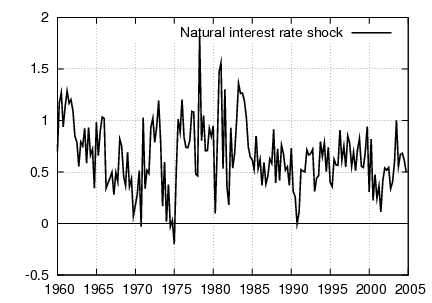
\includegraphics[scale=0.17]{/home/jmmurray/workspace/code/cfortran/initre_natint.png} & 
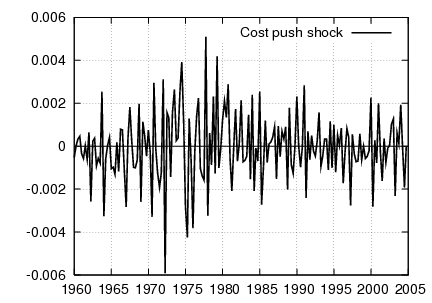
\includegraphics[scale=0.17]{/home/jmmurray/workspace/code/cfortran/initre_costpush.png} & 
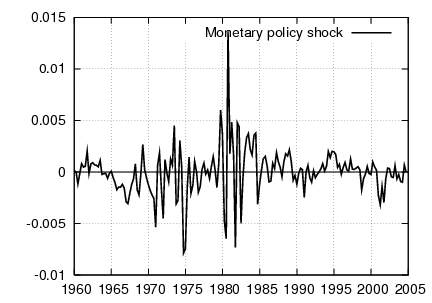
\includegraphics[scale=0.17]{/home/jmmurray/workspace/code/cfortran/initre_mpshock.png} \\ \\ 
\end{tabular}
}

\frame
{
  \ft{No Capital: Evolution of Shocks}
\begin{tabular}{ccc}
\multicolumn{3}{c}{Rational Expectations} \\ 
Nat. Rate & Cost Push & Policy Shock \\ 
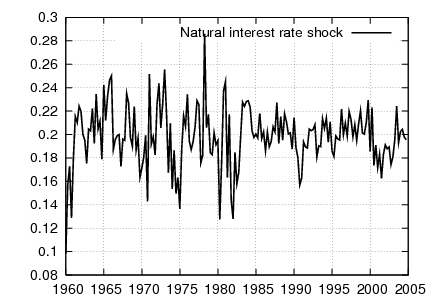
\includegraphics[scale=0.17]{/home/jmmurray/workspace/code/cfortran/re_natint.png} & 
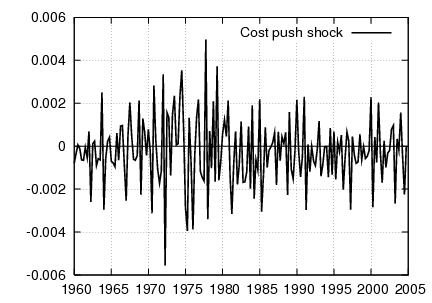
\includegraphics[scale=0.17]{/home/jmmurray/workspace/code/cfortran/re_costpush.png} & 
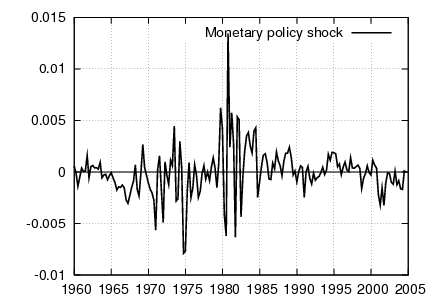
\includegraphics[scale=0.17]{/home/jmmurray/workspace/code/cfortran/re_mpshock.png} \\ \\ 
\multicolumn{3}{c}{Learning Without Observable Shocks} \\ 
Nat. Rate (0.9731) & Cost Push (0.9932) & Policy Shock (0.9995) \\ 
\includegraphics[scale=0.17]{/home/jmmurray/workspace/code/cfortran/initreg_natint.png} & 
\includegraphics[scale=0.17]{/home/jmmurray/workspace/code/cfortran/initreg_costpush.png} & 
\includegraphics[scale=0.17]{/home/jmmurray/workspace/code/cfortran/initreg_mpshock.png} \\ \\ 
\end{tabular}
}

\frame
{
  \ft{No Capital: Evolution of Shocks}
\begin{tabular}{ccc}
\multicolumn{3}{c}{Rational Expectations} \\ 
Nat. Rate & Cost Push & Policy Shock \\ 
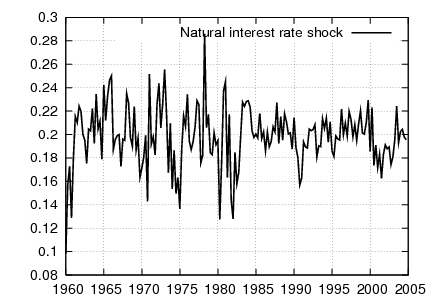
\includegraphics[scale=0.17]{/home/jmmurray/workspace/code/cfortran/re_natint.png} & 
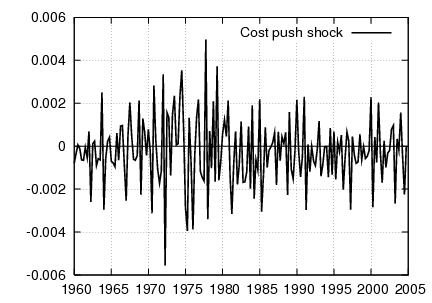
\includegraphics[scale=0.17]{/home/jmmurray/workspace/code/cfortran/re_costpush.png} & 
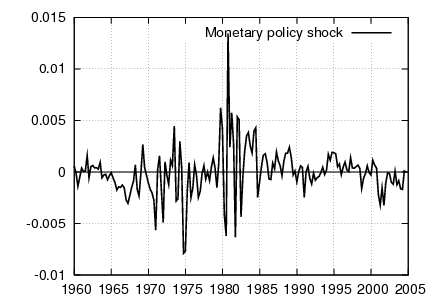
\includegraphics[scale=0.17]{/home/jmmurray/workspace/code/cfortran/re_mpshock.png} \\ \\ 
\multicolumn{3}{c}{Learning with Pre-sample Initial Conditions} \\ 
Nat. Rate (0.3652) & Cost Push (0.6110) & Policy Shock (0.9619) \\ 
\includegraphics[scale=0.17]{/home/jmmurray/workspace/code/cfortran/initwls_natint.png} & 
\includegraphics[scale=0.17]{/home/jmmurray/workspace/code/cfortran/initwls_costpush.png} & 
\includegraphics[scale=0.17]{/home/jmmurray/workspace/code/cfortran/initwls_mpshock.png} \\ \\ 
\end{tabular}
}

\frame
{
  \ft{No Capital: Evolution of Shocks}
\begin{tabular}{ccc}
\multicolumn{3}{c}{Rational Expectations} \\ 
Nat. Rate & Cost Push & Policy Shock \\ 
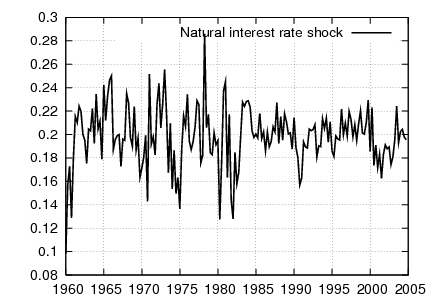
\includegraphics[scale=0.17]{/home/jmmurray/workspace/code/cfortran/re_natint.png} & 
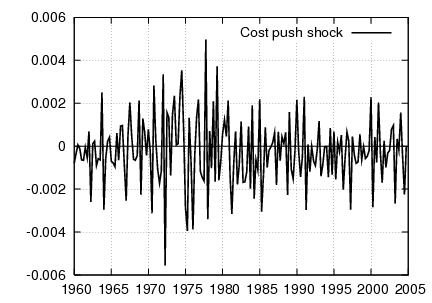
\includegraphics[scale=0.17]{/home/jmmurray/workspace/code/cfortran/re_costpush.png} & 
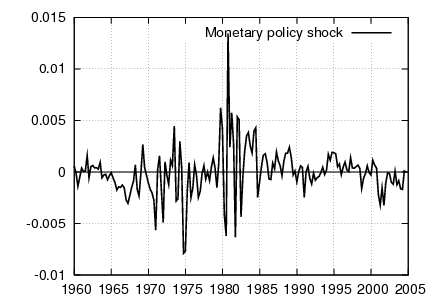
\includegraphics[scale=0.17]{/home/jmmurray/workspace/code/cfortran/re_mpshock.png} \\ \\ 
\multicolumn{3}{c}{Learning with Estimated Initial Conditions} \\ 
Nat. Rate (0.9769) & Cost Push (0.9832) & Policy Shock (0.9998) \\ 
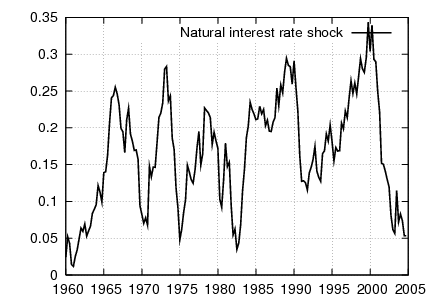
\includegraphics[scale=0.17]{/home/jmmurray/workspace/code/cfortran/initest_natint.png} & 
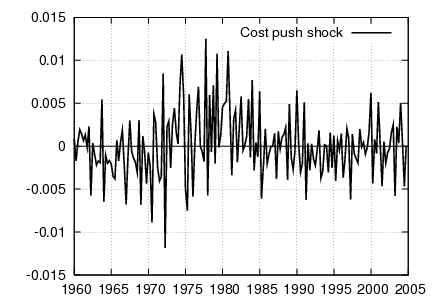
\includegraphics[scale=0.17]{/home/jmmurray/workspace/code/cfortran/initest_costpush.png} & 
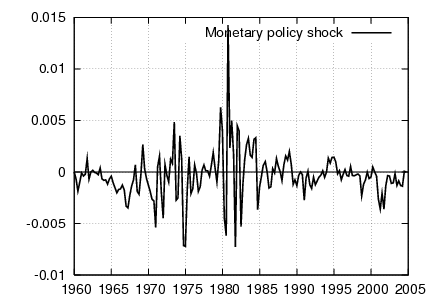
\includegraphics[scale=0.17]{/home/jmmurray/workspace/code/cfortran/initest_mpshock.png} \\ \\ 
\end{tabular}
}

\subsubsection{Evolution of Expectations}
\frame
{
  \ft{No Capital: Evolution of Expectations}
\begin{center}
\begin{tabular}{cc}
\multicolumn{2}{c}{Rational Expectations} \\ 
Output Gap & Inflation \\ 
\includegraphics[scale=0.17]{/home/jmmurray/workspace/code/cfortran/re_Expected_output_gap.png} & 
\includegraphics[scale=0.17]{/home/jmmurray/workspace/code/cfortran/re_Expected_inflation.png} \\ \\ 
\multicolumn{2}{c}{Learning with RE Initial Conditions} \\ 
Output Gap & Inflation \\ 
\includegraphics[scale=0.17]{/home/jmmurray/workspace/code/cfortran/initre_Expected_output_gap.png} & 
\includegraphics[scale=0.17]{/home/jmmurray/workspace/code/cfortran/initre_Expected_inflation.png} \\ \\ 
\end{tabular}
\end{center}
}


\frame
{
  \ft{No Capital: Evolution of Expectations}
\begin{center}
\begin{tabular}{cc}
\multicolumn{2}{c}{Rational Expectations} \\ 
Output Gap & Inflation \\ 
\includegraphics[scale=0.17]{/home/jmmurray/workspace/code/cfortran/re_Expected_output_gap.png} & 
\includegraphics[scale=0.17]{/home/jmmurray/workspace/code/cfortran/re_Expected_inflation.png} \\ \\ 
\multicolumn{2}{c}{Learning Without Using Shocks} \\ 
Output Gap & Inflation \\ 
\includegraphics[scale=0.17]{/home/jmmurray/workspace/code/cfortran/initreg_Expected_output_gap.png} & 
\includegraphics[scale=0.17]{/home/jmmurray/workspace/code/cfortran/initreg_Expected_inflation.png} \\ \\ 
\end{tabular}
\end{center}
}

\frame
{
  \ft{No Capital: Evolution of Expectations}
\begin{center}
\begin{tabular}{cc}
\multicolumn{2}{c}{Rational Expectations} \\ 
Output Gap & Inflation \\ 
\includegraphics[scale=0.17]{/home/jmmurray/workspace/code/cfortran/re_Expected_output_gap.png} & 
\includegraphics[scale=0.17]{/home/jmmurray/workspace/code/cfortran/re_Expected_inflation.png} \\ \\ 
\multicolumn{2}{c}{Learning with Pre-sample Initial Conditions} \\ 
Output Gap & Inflation \\ 
\includegraphics[scale=0.17]{/home/jmmurray/workspace/code/cfortran/initwls_Expected_output_gap.png} & 
\includegraphics[scale=0.17]{/home/jmmurray/workspace/code/cfortran/initwls_Expected_inflation.png} \\ \\ 
\end{tabular}
\end{center}
}

\frame
{
  \ft{No Capital: Evolution of Expectations}
\begin{center}
\begin{tabular}{cc}
\multicolumn{2}{c}{Rational Expectations} \\ 
Output Gap & Inflation \\ 
\includegraphics[scale=0.17]{/home/jmmurray/workspace/code/cfortran/re_Expected_output_gap.png} & 
\includegraphics[scale=0.17]{/home/jmmurray/workspace/code/cfortran/re_Expected_inflation.png} \\ \\ 
\multicolumn{2}{c}{Learning with Estimated Initial Conditions} \\ 
Output Gap & Inflation \\ 
\includegraphics[scale=0.17]{/home/jmmurray/workspace/code/cfortran/initest_Expected_output_gap.png} & 
\includegraphics[scale=0.17]{/home/jmmurray/workspace/code/cfortran/initest_Expected_inflation.png} \\ \\ 
\end{tabular}
\end{center}
}

\subsection{Model With Endogenous Capital}
\frame
{
\ft{Endogenous Capital: RE vs. Learning (RE Init.)}
\vspace*{-.15in}
\begin{center}
\begin{tiny}
\begin{tabular}{|l|c|rr|rr|} \hline
 \multicolumn{2}{|c|}{ } & \multicolumn{2}{|c|}{Case 1} & \multicolumn{2}{|c|}{Case 2} \\ \hline
Description & Parameter & Estimate & Std. Dev. & Estimate & Std. Dev. \\ \hline
Habit Formation & $\eta$ & 0.9181 & 0.1007 & 0.9181 & 0.1017 \\
Inverse IES & $\sigma$ & 0.3432 & 0.7774 & 0.3432 & 0.7967 \\
Capital Share & $\alpha$ & 0.3584 & 0.1189 & 0.3584 & 0.1219 \\
Cons / Output & $c_y$ & 0.8753 & 0.0044 & 0.8753 & 0.0044 \\
Cost Capital Adj. & $\phi$ & 6.9883 & 1.4836 & 6.9883 & 2.8850 \\
Phillips Slope & $\kappa$ & 0.0090 & 0.0036 & 0.0090 & 0.0039 \\
\hl{3}
Price Indexation & $\gamma$ & 0.0001 & 0.0768 & 0.0001 & 0.0769 \\
MP Persistence & $\rho_r$ & 0.7481 & 0.0472 & 0.7481 & 0.0570 \\
MP Output & $\psi_y$ & 0.1003 & 0.0379 & 0.1003 & 0.0379 \\
MP Inflation & $\psi_{\pi}$ & 1.0014 & 0.1195 & 1.0014 & 0.1219 \\
Tech. Shock Pers. & $\rho_z$ & 0.9716 & 0.0133 & 0.9716 & 0.0134 \\
Pref. Shock Pers. & $\rho_{\xi}$ & 0.5647 & 0.1159 & 0.5647 & 0.1160 \\
Inv. Shock Pers. & $\rho_{\mu}$ & 0.9050 & 0.0426 & 0.9050 & 0.0435 \\
Tech. Shock Std. Dev. & $\sigma_{z}$ & 0.0094 & 0.0041 & 0.0094 & 0.0044 \\
Inv. Shock Std. Dev. & $\sigma_{\mu}$ & 0.0306 & 0.0070 & 0.0306 & 0.0099 \\
Pref. Shock Std. Dev. & $\sigma_{\xi}$ & 0.3587 & 0.2699 & 0.3587 & 0.2741 \\
MP Shock Std. Dev. & $\sigma_r$ & 0.0033 & 0.0002 & 0.0033 & 0.0003 \\
SS Inflation & $\pi^{*}$ & 0.2209 & 4.2127 & 0.2209 & 4.2253 \\
SS Output (\$10,000) & $y^{*}$ & 1.4085 & 0.0212 & 1.4085 & 0.0213 \\
\hl{2}
Learning gain & $g$ & -- & -- & 0.0000 & 0.0147 \\\hline 
\multicolumn{2}{|l|}{Log-likelihood} & \multicolumn{2}{|r|}{-2391.5472} & \multicolumn{2}{|r|}{-2391.5472} \\ 
\multicolumn{2}{|l|}{MSE Consumption} & \multicolumn{2}{|r|}{7285.1049} & \multicolumn{2}{|r|}{7285.1049} \\ 
\multicolumn{2}{|l|}{MSE Investment} & \multicolumn{2}{|r|}{14454.2922} & \multicolumn{2}{|r|}{14454.2922} \\ 
\multicolumn{2}{|l|}{MSE Inflation} & \multicolumn{2}{|r|}{1.2633} & \multicolumn{2}{|r|}{1.2633} \\ 
\multicolumn{2}{|l|}{MSE Fed. Funds Rate} & \multicolumn{2}{|r|}{1.7499} & \multicolumn{2}{|r|}{1.7499} \\ \hline 
\end{tabular}
\end{tiny}
\end{center}
}

\frame
{
  \ft{Endogenous Capital: Forecast Errors}
\hspace*{-0.15in}
\begin{tabular}{cccc}
\multicolumn{4}{c}{Rational Expectations} \\ 
Consumption & Inflation & Fed. Funds & Investment \\ 
\includegraphics[scale=0.17]{/home/jmmurray/workspace/code/cfortran/cap_re_Forecast_error_consumption.png} & 
\includegraphics[scale=0.17]{/home/jmmurray/workspace/code/cfortran/cap_re_Forecast_error_inflation.png} & 
\includegraphics[scale=0.17]{/home/jmmurray/workspace/code/cfortran/cap_re_Forecast_error_Federal_Funds_rate.png} & 
\includegraphics[scale=0.17]{/home/jmmurray/workspace/code/cfortran/cap_re_Forecast_error_investment.png} \\ \\ 
\multicolumn{4}{c}{Learning with RE Initial Conditions} \\ 
Consumption  & Inflation  & Fed. Funds  & Investment \\ 
(1.0000) & (1.0000) & (1.0000) & (1.0000) \\ 
\includegraphics[scale=0.17]{/home/jmmurray/workspace/code/cfortran/cap_initre_Forecast_error_consumption.png} & 
\includegraphics[scale=0.17]{/home/jmmurray/workspace/code/cfortran/cap_initre_Forecast_error_inflation.png} & 
\includegraphics[scale=0.17]{/home/jmmurray/workspace/code/cfortran/cap_initre_Forecast_error_Federal_Funds_rate.png} & 
\includegraphics[scale=0.17]{/home/jmmurray/workspace/code/cfortran/cap_initre_Forecast_error_investment.png} \\ \\ 
\end{tabular}
}

\frame
{
\ft{Endogenous Capital: RE vs. Learning (No Shocks)}
\vspace*{-.15in}
\begin{center}
\begin{tiny}
\begin{tabular}{|l|c|rr|rr|} \hline
 \multicolumn{2}{|c|}{ } & \multicolumn{2}{|c|}{Case 1} & \multicolumn{2}{|c|}{Case 3} \\ \hline
Description & Parameter & Estimate & Std. Dev. & Estimate & Std. Dev. \\ \hline
Habit Formation & $\eta$ & 0.9181 & 0.1007 & 0.8393 & 0.1888 \\
Inverse IES & $\sigma$ & 0.3432 & 0.7774 & 0.3771 & 0.8493 \\
Capital Share & $\alpha$ & 0.3584 & 0.1189 & 0.3870 & 0.2697 \\
Cons / Output & $c_y$ & 0.8753 & 0.0044 & 0.8987 & 0.0000 \\
Cost Capital Adj. & $\phi$ & 6.9883 & 1.4836 & 6.9747 & 2.1739 \\
Phillips Slope & $\kappa$ & 0.0090 & 0.0036 & 0.0158 & 0.0065 \\
Price Indexation & $\gamma$ & 0.0001 & 0.0768 & 0.0007 & 0.0774 \\
MP Persistence & $\rho_r$ & 0.7481 & 0.0472 & 0.8031 & 0.0365 \\
MP Output & $\psi_y$ & 0.1003 & 0.0379 & 0.1005 & 0.0478 \\
MP Inflation & $\psi_{\pi}$ & 1.0014 & 0.1195 & 1.0285 & 0.1656 \\
Tech. Shock Pers. & $\rho_z$ & 0.9716 & 0.0133 & 0.9689 & 0.0461 \\
Pref. Shock Pers. & $\rho_{\xi}$ & 0.5647 & 0.1159 & 0.6644 & 0.1550 \\
Inv. Shock Pers. & $\rho_{\mu}$ & 0.9050 & 0.0426 & 0.9182 & 0.0050 \\
\hl{3}
Tech. Shock Std. Dev. & $\sigma_{z}$ & 0.0094 & 0.0041 & 0.1133 & 0.0708 \\
\hl{3}
Inv. Shock Std. Dev. & $\sigma_{\mu}$ & 0.0306 & 0.0070 & 0.1026 & 0.0189 \\
Pref. Shock Std. Dev. & $\sigma_{\xi}$ & 0.3587 & 0.2699 & 0.3532 & 0.1867 \\
MP Shock Std. Dev. & $\sigma_r$ & 0.0033 & 0.0002 & 0.0031 & 0.0001 \\
SS Inflation & $\pi^{*}$ & 0.2209 & 4.2127 & 3.8982 & 1.4266 \\
SS Output (\$10,000) & $y^{*}$ & 1.4085 & 0.0212 & 1.4200 & 0.0181 \\
\hl{2}
Learning gain & $g$ & -- & -- & 0.0052 & 0.0019 \\\hline 
\multicolumn{2}{|l|}{\hl{4}Log-likelihood} & \multicolumn{2}{|r|}{\hl{4}-2391.5472} & \multicolumn{2}{|r|}{\hl{4}-2320.0228} \\ 
\multicolumn{2}{|l|}{\hl{5}MSE Consumption} & \multicolumn{2}{|r|}{\hl{5}7285.1049} & \multicolumn{2}{|r|}{\hl{5}9532.5647} \\ 
\multicolumn{2}{|l|}{\hl{6}MSE Investment} & \multicolumn{2}{|r|}{\hl{6}14454.2922} & \multicolumn{2}{|r|}{\hl{6}11044.5295} \\ 
\multicolumn{2}{|l|}{\hl{7}MSE Inflation} & \multicolumn{2}{|r|}{\hl{7}1.2633} & \multicolumn{2}{|r|}{\hl{7}1.2455} \\ 
\multicolumn{2}{|l|}{\hl{7}MSE Fed. Funds Rate} & \multicolumn{2}{|r|}{\hl{7}1.7499} & \multicolumn{2}{|r|}{\hl{7}1.6766} \\ \hline 
\end{tabular}
\end{tiny}
\end{center}
}

\frame
{
  \ft{Endogenous Capital: Forecast Errors}
\hspace*{-0.15in}
\begin{tabular}{cccc}
\multicolumn{4}{c}{Rational Expectations} \\ 
Consumption & Inflation & Fed. Funds & Investment \\ 
\includegraphics[scale=0.17]{/home/jmmurray/workspace/code/cfortran/cap_re_Forecast_error_consumption.png} & 
\includegraphics[scale=0.17]{/home/jmmurray/workspace/code/cfortran/cap_re_Forecast_error_inflation.png} & 
\includegraphics[scale=0.17]{/home/jmmurray/workspace/code/cfortran/cap_re_Forecast_error_Federal_Funds_rate.png} & 
\includegraphics[scale=0.17]{/home/jmmurray/workspace/code/cfortran/cap_re_Forecast_error_investment.png} \\ \\ 
\multicolumn{4}{c}{Learning Without Observable Shocks} \\ 
Consumption & Inflation & Fed. Funds & Investment \\ 
 (0.9150) & (0.9635) & (0.9719) & (0.7828) \\
\includegraphics[scale=0.17]{/home/jmmurray/workspace/code/cfortran/cap_initreg_Forecast_error_consumption.png} & 
\includegraphics[scale=0.17]{/home/jmmurray/workspace/code/cfortran/cap_initreg_Forecast_error_inflation.png} & 
\includegraphics[scale=0.17]{/home/jmmurray/workspace/code/cfortran/cap_initreg_Forecast_error_Federal_Funds_rate.png} & 
\includegraphics[scale=0.17]{/home/jmmurray/workspace/code/cfortran/cap_initreg_Forecast_error_investment.png} \\ \\ 
\end{tabular}
}

\frame
{
\ft{Endogenous Capital: RE vs. Learning (Pre-sample)}
\vspace*{-.15in}
\begin{center}
\begin{tiny}
\begin{tabular}{|l|c|rr|rr|} \hline
 \multicolumn{2}{|c|}{ } & \multicolumn{2}{|c|}{Case 1} & \multicolumn{2}{|c|}{Case 4} \\ \hline
Description & Parameter & Estimate & Std. Dev. & Estimate & Std. Dev. \\ \hline
Habit Formation & $\eta$ & 0.9181 & 0.1007 & 0.7685 & 0.2555 \\
Inverse IES & $\sigma$ & 0.3432 & 0.7774 & 0.6433 & 1.7938 \\
Capital Share & $\alpha$ & 0.3584 & 0.1189 & 0.3177 & 0.3785 \\
Cons / Output & $c_y$ & 0.8753 & 0.0044 & 0.8944 & 0.0036 \\
Cost Capital Adj. & $\phi$ & 6.9883 & 1.4836 & 6.8234 & 2.6605 \\
Phillips Slope & $\kappa$ & 0.0090 & 0.0036 & 0.0113 & 0.0035 \\
Price Indexation & $\gamma$ & 0.0001 & 0.0768 & 0.0877 & 0.1071 \\
MP Persistence & $\rho_r$ & 0.7481 & 0.0472 & 0.8975 & 0.0382 \\
MP Output & $\psi_y$ & 0.1003 & 0.0379 & 0.1565 & 0.1132 \\
MP Inflation & $\psi_{\pi}$ & 1.0014 & 0.1195 & 1.0462 & 0.1866 \\
Tech. Shock Pers. & $\rho_z$ & 0.9716 & 0.0133 & 0.8205 & 0.0357 \\
\hl{3}
Pref. Shock Pers. & $\rho_{\xi}$ & 0.5647 & 0.1159 & 0.9007 & 0.0286 \\
Inv. Shock Pers. & $\rho_{\mu}$ & 0.9050 & 0.0426 & 0.9999 & 0.0000 \\
\hl{3}
Tech. Shock Std. Dev. & $\sigma_{z}$ & 0.0094 & 0.0041 & 0.3079 & 0.1910 \\
\hl{3}
Inv. Shock Std. Dev. & $\sigma_{\mu}$ & 0.0306 & 0.0070 & 0.1064 & 0.0133 \\
Pref. Shock Std. Dev. & $\sigma_{\xi}$ & 0.3587 & 0.2699 & 0.4362 & 0.4727 \\
MP Shock Std. Dev. & $\sigma_r$ & 0.0033 & 0.0002 & 0.0032 & 0.0001 \\
SS Inflation & $\pi^{*}$ & 0.2209 & 4.2127 & 0.0035 & 0.9250 \\
SS Output (\$10,000) & $y^{*}$ & 1.4085 & 0.0212 & 1.4074 & 0.0089 \\
\hl{2}
Learning gain & $g$ & -- & -- & 0.0060 & 0.0012 \\\hline 
\multicolumn{2}{|l|}{\hl{4}Log-likelihood} & \multicolumn{2}{|r|}{\hl{4}-2391.5472} & \multicolumn{2}{|r|}{\hl{4}-2506.8255} \\ 
\multicolumn{2}{|l|}{\hl{4}MSE Consumption} & \multicolumn{2}{|r|}{\hl{4}7285.1049} & \multicolumn{2}{|r|}{\hl{4}9584.1202} \\ 
\multicolumn{2}{|l|}{\hl{4}MSE Investment} & \multicolumn{2}{|r|}{\hl{4}14454.2922} & \multicolumn{2}{|r|}{\hl{4}44510.7805} \\ 
\multicolumn{2}{|l|}{\hl{4}MSE Inflation} & \multicolumn{2}{|r|}{\hl{4}1.2633} & \multicolumn{2}{|r|}{\hl{4}3.5212} \\ 
\multicolumn{2}{|l|}{\hl{4}MSE Fed. Funds Rate} & \multicolumn{2}{|r|}{\hl{4}1.7499} & \multicolumn{2}{|r|}{\hl{4}1.5378} \\ \hline 
\end{tabular}
\end{tiny}
\end{center}
}

\frame
{
  \ft{Endogenous Capital: Forecast Errors}
\hspace*{-0.15in}
\begin{tabular}{cccc}
\multicolumn{4}{c}{Rational Expectations} \\ 
Consumption & Inflation & Fed. Funds & Investment \\ 
\includegraphics[scale=0.17]{/home/jmmurray/workspace/code/cfortran/cap_re_Forecast_error_consumption.png} & 
\includegraphics[scale=0.17]{/home/jmmurray/workspace/code/cfortran/cap_re_Forecast_error_inflation.png} & 
\includegraphics[scale=0.17]{/home/jmmurray/workspace/code/cfortran/cap_re_Forecast_error_Federal_Funds_rate.png} & 
\includegraphics[scale=0.17]{/home/jmmurray/workspace/code/cfortran/cap_re_Forecast_error_investment.png} \\ \\
\multicolumn{4}{c}{Learning with Pre-sample Initial Conditions} \\ 
Consumption & Inflation & Fed. Funds & Investment \\ 
(0.8813) & (0.6142) & (0.9301) & (0.5128) \\
\includegraphics[scale=0.17]{/home/jmmurray/workspace/code/cfortran/cap_initwls_Forecast_error_consumption.png} & 
\includegraphics[scale=0.17]{/home/jmmurray/workspace/code/cfortran/cap_initwls_Forecast_error_inflation.png} & 
\includegraphics[scale=0.17]{/home/jmmurray/workspace/code/cfortran/cap_initwls_Forecast_error_Federal_Funds_rate.png} & 
\includegraphics[scale=0.17]{/home/jmmurray/workspace/code/cfortran/cap_initwls_Forecast_error_investment.png} \\ \\ 
\end{tabular}
}


\frame
{
\ft{Endogenous Capital: RE vs. Learning (Estimated)}
\vspace*{-.15in}
\begin{center}
\begin{tiny}
\begin{tabular}{|l|c|rr|rr|} \hline
 \multicolumn{2}{|c|}{ } & \multicolumn{2}{|c|}{Case 1} & \multicolumn{2}{|c|}{Case 5} \\ \hline
Description & Parameter & Estimate & Std. Dev. & Estimate & Std. Dev. \\ \hline
\hl{3}
Habit Formation & $\eta$ & 0.9181 & 0.1007 & 0.8564 & 6.7771 \\
\hl{3}
Inverse IES & $\sigma$ & 0.3432 & 0.7774 & 0.1667 & 16.3052 \\
Capital Share & $\alpha$ & 0.3584 & 0.1189 & 0.3662 & 0.6600 \\
Cons / Output & $c_y$ & 0.8753 & 0.0044 & 0.8851 & 0.0122 \\
Cost Capital Adj. & $\phi$ & 6.9883 & 1.4836 & 6.9999 & 0.0001 \\
Phillips Slope & $\kappa$ & 0.0090 & 0.0036 & 0.0287 & 0.0201 \\
\hl{3}
Price Indexation & $\gamma$ & 0.0001 & 0.0768 & 0.0002 & 0.3186 \\
MP Persistence & $\rho_r$ & 0.7481 & 0.0472 & 0.9136 & 0.0641 \\
MP Output & $\psi_y$ & 0.1003 & 0.0379 & 0.1296 & 0.2032 \\
MP Inflation & $\psi_{\pi}$ & 1.0014 & 0.1195 & 1.0089 & 0.4514 \\
Tech. Shock Pers. & $\rho_z$ & 0.9716 & 0.0133 & 0.9582 & 0.0411 \\
Pref. Shock Pers. & $\rho_{\xi}$ & 0.5647 & 0.1159 & 0.1614 & 0.1110 \\
Inv. Shock Pers. & $\rho_{\mu}$ & 0.9050 & 0.0426 & 0.9075 & 0.0902 \\
Tech. Shock Std. Dev. & $\sigma_{z}$ & 0.0094 & 0.0041 & 0.0609 & 0.0920 \\
Inv. Shock Std. Dev. & $\sigma_{\mu}$ & 0.0306 & 0.0070 & 0.0709 & 0.0220 \\
Pref. Shock Std. Dev. & $\sigma_{\xi}$ & 0.3587 & 0.2699 & 0.0918 & 0.2118 \\
MP Shock Std. Dev. & $\sigma_r$ & 0.0033 & 0.0002 & 0.0030 & 0.0001 \\
SS Inflation & $\pi^{*}$ & 0.2209 & 4.2127 & 0.2202 & 4.7265 \\
SS Output (\$10,000) & $y^{*}$ & 1.4085 & 0.0212 & 1.4177 & 0.0783 \\
\hl{2}
Learning gain & $g$ & -- & -- & 0.0005 & 0.0018 \\\hline 
\multicolumn{2}{|l|}{\hl{4}Log-likelihood} & \multicolumn{2}{|r|}{\hl{4}-2391.5472} & \multicolumn{2}{|r|}{\hl{4}-2237.0404} \\ 
\multicolumn{2}{|l|}{\hl{4}MSE Consumption} & \multicolumn{2}{|r|}{\hl{4}7285.1049} & \multicolumn{2}{|r|}{\hl{4}6702.3679} \\ 
\multicolumn{2}{|l|}{\hl{5}MSE Investment} & \multicolumn{2}{|r|}{\hl{5}14454.2922} & \multicolumn{2}{|r|}{\hl{5}6304.4836} \\ 
\multicolumn{2}{|l|}{\hl{4}MSE Inflation} & \multicolumn{2}{|r|}{\hl{4}1.2633} & \multicolumn{2}{|r|}{\hl{4}1.1815} \\ 
\multicolumn{2}{|l|}{\hl{4}MSE Fed. Funds Rate} & \multicolumn{2}{|r|}{\hl{4}1.7499} & \multicolumn{2}{|r|}{\hl{4}1.4896} \\ \hline 
\end{tabular}
\end{tiny}
\end{center}
}

\frame
{
  \ft{Endogenous Capital: Forecast Errors}
\hspace*{-0.15in}
\begin{tabular}{cccc}
\multicolumn{4}{c}{Rational Expectations} \\ 
Consumption & Inflation & Fed. Funds & Investment \\ 
\includegraphics[scale=0.17]{/home/jmmurray/workspace/code/cfortran/cap_re_Forecast_error_consumption.png} & 
\includegraphics[scale=0.17]{/home/jmmurray/workspace/code/cfortran/cap_re_Forecast_error_inflation.png} & 
\includegraphics[scale=0.17]{/home/jmmurray/workspace/code/cfortran/cap_re_Forecast_error_Federal_Funds_rate.png} & 
\includegraphics[scale=0.17]{/home/jmmurray/workspace/code/cfortran/cap_re_Forecast_error_investment.png} \\ \\
\multicolumn{4}{c}{Learning with Estimated Initial Conditions} \\ 
Consumption & Inflation & Fed. Funds & Investment \\ 
(0.8977) & (0.9843) & (0.9245) & (0.6910) \\
\includegraphics[scale=0.17]{/home/jmmurray/workspace/code/cfortran/cap_initest_Forecast_error_consumption.png} & 
\includegraphics[scale=0.17]{/home/jmmurray/workspace/code/cfortran/cap_initest_Forecast_error_inflation.png} & 
\includegraphics[scale=0.17]{/home/jmmurray/workspace/code/cfortran/cap_initest_Forecast_error_Federal_Funds_rate.png} & 
\includegraphics[scale=0.17]{/home/jmmurray/workspace/code/cfortran/cap_initest_Forecast_error_investment.png} \\ \\ 
\end{tabular}
}

\subsubsection{Evolution of Shocks}
\frame
{
  \ft{Endogenous Capital: Evolution of Shocks}
\hspace*{-0.15in}
\begin{tabular}{cccc}
\multicolumn{4}{c}{Rational Expectations} \\ 
Preference & Technology & Investment & Policy Shock \\ 
\includegraphics[scale=0.17]{/home/jmmurray/workspace/code/cfortran/cap_re_prefsh.png} & 
\includegraphics[scale=0.17]{/home/jmmurray/workspace/code/cfortran/cap_re_techsh.png} & 
\includegraphics[scale=0.17]{/home/jmmurray/workspace/code/cfortran/cap_re_invsh.png} & 
\includegraphics[scale=0.17]{/home/jmmurray/workspace/code/cfortran/cap_re_mpshock.png} \\ \\ 
\multicolumn{4}{c}{Learning with RE Initial Conditions} \\ 
Preference & Technology & Investment & Policy Shock \\ 
(1.0000) & (1.0000) & (1.0000) & (1.0000) \\
\includegraphics[scale=0.17]{/home/jmmurray/workspace/code/cfortran/cap_initre_prefsh.png} & 
\includegraphics[scale=0.17]{/home/jmmurray/workspace/code/cfortran/cap_initre_techsh.png} & 
\includegraphics[scale=0.17]{/home/jmmurray/workspace/code/cfortran/cap_initre_invsh.png} & 
\includegraphics[scale=0.17]{/home/jmmurray/workspace/code/cfortran/cap_initre_mpshock.png} \\ \\ 
\end{tabular}
}


\frame
{
  \ft{Endogenous Capital: Evolution of Shocks}
\hspace*{-0.15in}
\begin{tabular}{cccc}
\multicolumn{4}{c}{Rational Expectations} \\ 
Preference & Technology & Investment & Policy Shock \\ 
\includegraphics[scale=0.17]{/home/jmmurray/workspace/code/cfortran/cap_re_prefsh.png} & 
\includegraphics[scale=0.17]{/home/jmmurray/workspace/code/cfortran/cap_re_techsh.png} & 
\includegraphics[scale=0.17]{/home/jmmurray/workspace/code/cfortran/cap_re_invsh.png} & 
\includegraphics[scale=0.17]{/home/jmmurray/workspace/code/cfortran/cap_re_mpshock.png} \\ \\ 
\multicolumn{4}{c}{Learning Without Observable Shocks} \\ 
Preference & Technology & Investment & Policy Shock \\ 
(0.8697) & (0.6534) & (-0.8120) & (0.9867) \\
\includegraphics[scale=0.17]{/home/jmmurray/workspace/code/cfortran/cap_initreg_prefsh.png} & 
\includegraphics[scale=0.17]{/home/jmmurray/workspace/code/cfortran/cap_initreg_techsh.png} & 
\includegraphics[scale=0.17]{/home/jmmurray/workspace/code/cfortran/cap_initreg_invsh.png} & 
\includegraphics[scale=0.17]{/home/jmmurray/workspace/code/cfortran/cap_initreg_mpshock.png} \\ \\ 
\end{tabular}
}

\frame
{
  \ft{Endogenous Capital: Evolution of Shocks}
\hspace*{-0.15in}
\begin{tabular}{cccc}
\multicolumn{4}{c}{Rational Expectations} \\ 
Preference & Technology & Investment & Policy Shock \\ 
\includegraphics[scale=0.17]{/home/jmmurray/workspace/code/cfortran/cap_re_prefsh.png} & 
\includegraphics[scale=0.17]{/home/jmmurray/workspace/code/cfortran/cap_re_techsh.png} & 
\includegraphics[scale=0.17]{/home/jmmurray/workspace/code/cfortran/cap_re_invsh.png} & 
\includegraphics[scale=0.17]{/home/jmmurray/workspace/code/cfortran/cap_re_mpshock.png} \\ \\ 
\multicolumn{4}{c}{Learning with Pre-sample Initial Conditions} \\ 
Preference & Technology & Investment & Policy Shock \\ 
(0.7522) & (0.5440) & (-0.6584) & (0.8697) \\
\includegraphics[scale=0.17]{/home/jmmurray/workspace/code/cfortran/cap_initwls_prefsh.png} & 
\includegraphics[scale=0.17]{/home/jmmurray/workspace/code/cfortran/cap_initwls_techsh.png} & 
\includegraphics[scale=0.17]{/home/jmmurray/workspace/code/cfortran/cap_initwls_invsh.png} & 
\includegraphics[scale=0.17]{/home/jmmurray/workspace/code/cfortran/cap_initwls_mpshock.png} \\ \\ 
\end{tabular}
}


\frame
{
  \ft{Endogenous Capital: Evolution of Shocks}
\hspace*{-0.15in}
\begin{tabular}{cccc}
\multicolumn{4}{c}{Rational Expectations} \\ 
Preference & Technology & Investment & Policy Shock \\ 
\includegraphics[scale=0.17]{/home/jmmurray/workspace/code/cfortran/cap_re_prefsh.png} & 
\includegraphics[scale=0.17]{/home/jmmurray/workspace/code/cfortran/cap_re_techsh.png} & 
\includegraphics[scale=0.17]{/home/jmmurray/workspace/code/cfortran/cap_re_invsh.png} & 
\includegraphics[scale=0.17]{/home/jmmurray/workspace/code/cfortran/cap_re_mpshock.png} \\ \\ 
\multicolumn{4}{c}{Learning with Estimated Initial Conditions} \\ 
Preference & Technology & Investment & Policy Shock \\ 
(0.8200) & (0.8365) & (-0.7371) & (0.8917) \\
\includegraphics[scale=0.17]{/home/jmmurray/workspace/code/cfortran/cap_initest_prefsh.png} & 
\includegraphics[scale=0.17]{/home/jmmurray/workspace/code/cfortran/cap_initest_techsh.png} & 
\includegraphics[scale=0.17]{/home/jmmurray/workspace/code/cfortran/cap_initest_invsh.png} & 
\includegraphics[scale=0.17]{/home/jmmurray/workspace/code/cfortran/cap_initest_mpshock.png} \\ \\ 

\end{tabular}
}

\subsubsection{Evolution of Expectations}

\frame
{
  \ft{Endogenous Capital: Evolution of Expectations}
  \hspace*{-0.15in}
\begin{tabular}{cccc}
\multicolumn{4}{c}{Rational Expectations} \\ 
Consumption & Inflation & Capital Stock & Output \\ 
\includegraphics[scale=0.17]{/home/jmmurray/workspace/code/cfortran/cap_re_Expected_consumption.png} & 
\includegraphics[scale=0.17]{/home/jmmurray/workspace/code/cfortran/cap_re_Expected_inflation.png} & 
\includegraphics[scale=0.17]{/home/jmmurray/workspace/code/cfortran/cap_re_Expected_capital.png} & 
\includegraphics[scale=0.17]{/home/jmmurray/workspace/code/cfortran/cap_re_Expected_output.png} \\ \\ 
\multicolumn{4}{c}{Learning with RE Initial Conditions} \\ 
Consumption & Inflation & Capital Stock & Output \\ 
\includegraphics[scale=0.17]{/home/jmmurray/workspace/code/cfortran/cap_initre_Expected_consumption.png} & 
\includegraphics[scale=0.17]{/home/jmmurray/workspace/code/cfortran/cap_initre_Expected_inflation.png} & 
\includegraphics[scale=0.17]{/home/jmmurray/workspace/code/cfortran/cap_initre_Expected_capital.png} & 
\includegraphics[scale=0.17]{/home/jmmurray/workspace/code/cfortran/cap_initre_Expected_output.png} \\ \\ 
\end{tabular}
}

\frame
{
  \ft{Endogenous Capital: Evolution of Expectations}
  \hspace*{-0.15in}
\begin{tabular}{cccc}
\multicolumn{4}{c}{Rational Expectations} \\ 
Consumption & Inflation & Capital Stock & Output \\ 
\includegraphics[scale=0.17]{/home/jmmurray/workspace/code/cfortran/cap_re_Expected_consumption.png} & 
\includegraphics[scale=0.17]{/home/jmmurray/workspace/code/cfortran/cap_re_Expected_inflation.png} & 
\includegraphics[scale=0.17]{/home/jmmurray/workspace/code/cfortran/cap_re_Expected_capital.png} & 
\includegraphics[scale=0.17]{/home/jmmurray/workspace/code/cfortran/cap_re_Expected_output.png} \\ \\ 
\multicolumn{4}{c}{Learning Without Using Shocks} \\ 
Consumption & Inflation & Capital Stock & Output \\ 
\includegraphics[scale=0.17]{/home/jmmurray/workspace/code/cfortran/cap_initreg_Expected_consumption.png} & 
\includegraphics[scale=0.17]{/home/jmmurray/workspace/code/cfortran/cap_initreg_Expected_inflation.png} & 
\includegraphics[scale=0.17]{/home/jmmurray/workspace/code/cfortran/cap_initreg_Expected_capital.png} & 
\includegraphics[scale=0.17]{/home/jmmurray/workspace/code/cfortran/cap_initreg_Expected_output.png} \\ \\ 
\end{tabular}
}

\frame
{
  \ft{Endogenous Capital: Evolution of Expectations}
  \hspace*{-0.15in}
\begin{tabular}{cccc}
\multicolumn{4}{c}{Rational Expectations} \\ 
Consumption & Inflation & Capital Stock & Output \\ 
\includegraphics[scale=0.17]{/home/jmmurray/workspace/code/cfortran/cap_re_Expected_consumption.png} & 
\includegraphics[scale=0.17]{/home/jmmurray/workspace/code/cfortran/cap_re_Expected_inflation.png} & 
\includegraphics[scale=0.17]{/home/jmmurray/workspace/code/cfortran/cap_re_Expected_capital.png} & 
\includegraphics[scale=0.17]{/home/jmmurray/workspace/code/cfortran/cap_re_Expected_output.png} \\ \\ 
\multicolumn{4}{c}{Learning with Pre-sample Initial Conditions} \\ 
Consumption & Inflation & Capital Stock & Output \\ 
\includegraphics[scale=0.17]{/home/jmmurray/workspace/code/cfortran/cap_initwls_Expected_consumption.png} & 
\includegraphics[scale=0.17]{/home/jmmurray/workspace/code/cfortran/cap_initwls_Expected_inflation.png} & 
\includegraphics[scale=0.17]{/home/jmmurray/workspace/code/cfortran/cap_initwls_Expected_capital.png} & 
\includegraphics[scale=0.17]{/home/jmmurray/workspace/code/cfortran/cap_initwls_Expected_output.png} \\ \\ 
\end{tabular}
}

\frame
{
  \ft{Endogenous Capital: Evolution of Expectations}
  \hspace*{-0.15in}
\begin{tabular}{cccc}
\multicolumn{4}{c}{Rational Expectations} \\ 
Consumption & Inflation & Capital Stock & Output \\ 
\includegraphics[scale=0.17]{/home/jmmurray/workspace/code/cfortran/cap_re_Expected_consumption.png} & 
\includegraphics[scale=0.17]{/home/jmmurray/workspace/code/cfortran/cap_re_Expected_inflation.png} & 
\includegraphics[scale=0.17]{/home/jmmurray/workspace/code/cfortran/cap_re_Expected_capital.png} & 
\includegraphics[scale=0.17]{/home/jmmurray/workspace/code/cfortran/cap_re_Expected_output.png} \\ \\ 
\multicolumn{4}{c}{Learning with Estimated Initial Conditions} \\ 
Consumption & Inflation & Capital Stock & Output \\ 
\includegraphics[scale=0.17]{/home/jmmurray/workspace/code/cfortran/cap_initest_Expected_consumption.png} & 
\includegraphics[scale=0.17]{/home/jmmurray/workspace/code/cfortran/cap_initest_Expected_inflation.png} & 
\includegraphics[scale=0.17]{/home/jmmurray/workspace/code/cfortran/cap_initest_Expected_capital.png} & 
\includegraphics[scale=0.17]{/home/jmmurray/workspace/code/cfortran/cap_initest_Expected_output.png} \\ \\ 
\end{tabular}
}

\section{}
\subsection{Conclusion}
\frame
{
  \ft{Conclusion}
  \bi
  \item<+-> Summary of findings:
    \bi
    \item<+-> Learning does not better explain data.
    \item<+-> No capital: negligible differences in forecast errors, shocks, and expectations.
    \item<+-> Making shocks unobservable causes MLE to predict more volatile shocks.
    \item<+-> Best fitting models: Learning without observable shocks.
    \item<+-> Worst fitting models: Pre-sample initial conditions.
    \item<+-> Unobservable shocks creates less volatile expectations.
    \item<+-> Learning expectations about capital stock causes opposite predictions for investment shocks.
    \ei
  \item<+-> Learning failures:
    \bi
    \item<+-> Fails to explain persistence.
    \item<+-> Fails to explain Great Inflation / Great Moderation.
    \ei
  \ei
}


\end{document}
